\newpage
\section{THIẾT KẾ HỆ THỐNG}
\subsection{Tổng quan hệ thống}

\textbf{Thiết bị sử dụng}
- The **Micro:bit** acts as the core microcontroller,      reading data from sensors and controlling actuators.
- Sensors detect security-related events (e.g., motion,      temperature, door status).
- Actuators (e.g., alarms, lights, locks) respond to      user commands.
- The Micro:bit communicates with a computer via **serial      connection (USB or Bluetooth).**


\begin{figure}[H]
    \centering
    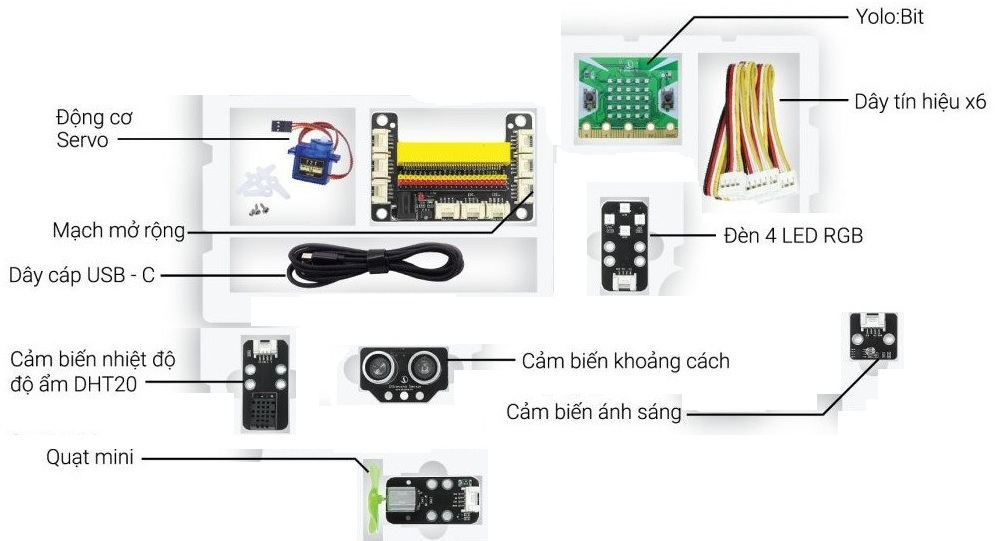
\includegraphics[width=0.7\textwidth]{selected_device.jpg}
    \caption{Các thiết bị được chọn sử dụng trong hệ thống}
    \label{fig:selected_device}
\end{figure}

\textbf{Thiết bị đầu vào}
Cảm biến nhiệt độ độ ẩm DHT20
\begin{itemize}
    \item \textbf{Ứng dụng}: Đo nhiệt độ và độ ẩm trong môi trường. Hiển thị dữ liệu lên màn hình LCD. Kích hoạt quạt mini nếu nhiệt độ vượt quá ngưỡng cài đặt.
    \item \textbf{Đầu vào}: Nhiệt độ, độ ẩm - cảm biến được đặt trong môi trường giám sát.
    \item \textbf{Đầu ra}: Giá trị nhiệt độ, độ ẩm được gửi đến vi điều khiển và hiển thị trên màn hình LCD.
\end{itemize}

Cảm biến khoảng cách hồng ngoại
\begin{itemize}
    \item \textbf{Ứng dụng}: Phát hiện vật thể trong phạm vi nhất định. Khi phát hiện người xâm nhập, kích hoạt báo động bằng đèn LED RGB hoặc hiển thị cảnh báo lên màn hình LCD.
    \item \textbf{Đầu vào}: Khoảng cách - cảm biến được lắp đặt tại vị trí giám sát.
    \item \textbf{Đầu ra}: Tín hiệu phát hiện chuyển động được gửi đến vi điều khiển để xử lý.
\end{itemize}

Cảm biến ánh sáng
\begin{itemize}
    \item \textbf{Ứng dụng}: Đo mức độ ánh sáng môi trường. Khi trời tối, hệ thống có thể tự động bật đèn LED RGB và tắt khi trời sáng.
    \item \textbf{Đầu vào}: Cường độ ánh sáng - cảm biến được đặt tại môi trường ngoài trời hoặc trong phòng.
    \item \textbf{Đầu ra}: Tín hiệu cường độ ánh sáng được xử lý để điều khiển LED RGB.
\end{itemize}

\textbf{Thiết bị đầu ra}
Động cơ Servo
\begin{itemize}
    \item \textbf{Ứng dụng}: Điều khiển cửa tự động đóng/mở khi có tín hiệu từ remote hoặc cảm biến khoảng cách.
    \item \textbf{Đầu vào}: Tín hiệu điều khiển từ vi điều khiển.
    \item \textbf{Đầu ra}: Thay đổi góc mở cửa theo tín hiệu điều khiển.
\end{itemize}

Đèn 4 LED RGB
\begin{itemize}
    \item \textbf{Ứng dụng}: Hiển thị trạng thái hệ thống (xanh: bình thường, đỏ: cảnh báo, nhấp nháy: báo động). Bật sáng khi trời tối và tắt khi trời sáng. Nhấp nháy khi có cảnh báo từ cảm biến khoảng cách hoặc nhiệt độ cao.
    \item \textbf{Đầu vào}: Tín hiệu điều khiển từ vi điều khiển.
    \item \textbf{Đầu ra}: Phát sáng theo màu sắc quy định.
\end{itemize}


Quạt mini
\begin{itemize}
    \item \textbf{Ứng dụng}: Kích hoạt khi nhiệt độ vượt quá ngưỡng cài đặt (ví dụ: trên $30 C$). Có thể bật/tắt từ remote.
    \item \textbf{Đầu vào}: Tín hiệu từ vi điều khiển hoặc người dùng.
    \item \textbf{Đầu ra}: Quạt hoạt động để làm mát môi trường.
\end{itemize}

\textbf{Các thiết bị khác}
Yolo:Bit
\begin{itemize}
    \item \textbf{Ứng dụng}: Vi điều khiển chính của hệ thống, xử lý dữ liệu từ cảm biến và điều khiển thiết bị đầu ra.
    \item \textbf{Đầu vào}: Dữ liệu từ các cảm biến.
    \item \textbf{Đầu ra}: Tín hiệu điều khiển thiết bị ngoại vi.
\end{itemize}

Mạch mở rộng
\begin{itemize}
    \item \textbf{Ứng dụng}: Kết nối và cấp nguồn cho các thiết bị ngoại vi như cảm biến, động cơ, màn hình LCD, LED RGB.
    \item \textbf{Đầu vào}: Nguồn điện từ USB hoặc pin.
    \item \textbf{Đầu ra}: Phân phối nguồn và kết nối tín hiệu giữa các thiết bị.
\end{itemize}

Dây tín hiệu x6
\begin{itemize}
    \item \textbf{Ứng dụng}: Truyền tín hiệu giữa Yolo:Bit và các thiết bị ngoại vi.
    \item \textbf{Đầu vào}: Kết nối giữa vi điều khiển và thiết bị ngoại vi.
    \item \textbf{Đầu ra}: Truyền dữ liệu và tín hiệu điều khiển.
\end{itemize}

Dây cáp USB-C
\begin{itemize}
    \item \textbf{Ứng dụng}: Cấp nguồn và lập trình cho Yolo:Bit.
    \item \textbf{Đầu vào}: Nguồn điện từ adapter hoặc máy tính.
    \item \textbf{Đầu ra}: Cấp điện và truyền dữ liệu lập trình.
\end{itemize}

1. **Computer-side Python Script (Edge Processing \&     Cloud Communication)**
- Runs on a PC connected to the Micro:bit.
- Collects sensor data from the Micro:bit and sends it      to the **Adafruit IO server**.
- Retrieves commands from the Adafruit IO server and      forwards them to the Micro:bit.
- Ensures real-time logging and processing of sensor data.
2. **Web Application (User Interface \& Remote Control)**
- Allows users to **view live sensor data** and **send      commands** to actuators.
- Connects directly to **Adafruit IO** for real-time      data fetching and command sending.
- Uses **Firebase** for user authentication and      actuator list management.
3. **Firebase (User Management \& Device Configuration)**
- Stores user accounts, authentication details, and      access permissions.
- Maintains a list of registered actuators that each      user can control.
- Ensures secure access by verifying user identity      before allowing device interaction.

\textbf{Data Flow and Command Flow}

Cập nhật dữ liệu mỗi 100ms

1. **Data Flow (Sensor to Web UI)**
- Micro:bit reads data from sensors.
- Sends data to the **Python script** on the computer      via serial communication.
- Python script **uploads the data to Adafruit IO**.
- The web app fetches the data from Adafruit IO and      displays it.
2. **Command Flow (User to Actuator)**
- User sends a command via the web application.
- The command is **stored in Adafruit IO**.
- The Python script running on the computer fetches the      command.
- It sends the command to the Micro:bit, which **activates      the appropriate actuator**.




\subsection{Công nghệ sử dụng}
- React Native: Mobile App
- ExpressJS: xây dựng API
- Firebase
- Google Cloud Service: API Text To Speech
- YoloV8: AI Hình ảnh
- Adafruit
**Micro:bit** - Handles sensors \& actuators
**Python (Computer-side Script)** - Manages communication with Micro:bit \& Adafruit
**Adafruit IO** - Cloud IoT service for data logging \& command relay
**Firebase** - User authentication \& actuator list storage
**Web Technologies (HTML, CSS, JS)** - User interface for remote monitoring \& control
Figma, Photoshop thiết kế giao diện cho web app
**Các hình ảnh diagram trong báo cáo vẽ bằng Lucidchart**
Báo cáo trên Overleaf
Github lưu trữ mã nguồn
host trang web này bằng github page